	% Copyright 2004 by Till Tantau <tantau@users.sourceforge.net>.
%
% In principle, this file can be redistributed and/or modified under
% the terms of the GNU Public License, version 2.
%
% However, this file is supposed to be a template to be modified
% for your own needs. For this reason, if you use this file as a
% template and not specifically distribute it as part of a another
% package/program, I grant the extra permission to freely copy and
% modify this file as you see fit and even to delete this copyright
% notice. 

\documentclass{beamer}

% There are many different themes available for Beamer. A comprehensive
% list with examples is given here:
% http://deic.uab.es/~iblanes/beamer_gallery/index_by_theme.html
% You can uncomment the themes below if you would like to use a different
% one:
%\usetheme{AnnArbor}
%\usetheme{Antibes}
%\usetheme{Bergen}
%\usetheme{Berkeley}
%\usetheme{Berlin}
%\usetheme{Boadilla}
%\usetheme{boxes}
%\usetheme{CambridgeUS}
%\usetheme{Copenhagen}
%\usetheme{Darmstadt}
%\usetheme{default}
%\usetheme{Frankfurt}
%\usetheme{Goettingen}
%\usetheme{Hannover}
%\usetheme{Ilmenau}
%\usetheme{JuanLesPins}
%\usetheme{Luebeck}
\usetheme{Madrid}
%\usetheme{Malmoe}
%\usetheme{Marburg}
%\usetheme{Montpellier}
%\usetheme{PaloAlto}
%\usetheme{Pittsburgh}
%\usetheme{Rochester}
%\usetheme{Singapore}
%\usetheme{Szeged}
%\usetheme{Warsaw}

\usepackage{media9}
\usepackage{ragged2e}
\usepackage{tikz}
\usepackage{epstopdf}
\usepackage{algorithm2e}
%from videos tutorial
\usepackage[utf8]{inputenc}
\usepackage[T1]{fontenc}
\usepackage{parskip}

\usepackage{graphicx}
\usepackage{media9}
%\usepackage{algorithm}

% Customize Warsaw color 
\setbeamercolor*{palette primary}{use=structure,fg=white,bg=red!50!black}
\setbeamercolor*{palette secondary}{use=structure,fg=white,bg=red!60!black}
\setbeamercolor*{palette tertiary}{use=structure,fg=white,bg=red!70!black}
\part{First Presentation}
% Customize Warsaw block title and background colors
\setbeamertemplate{section in toc}[ball unnumbered]
\setbeamercolor{block title}{bg=red!50!black,fg=white}

\title{Model Free Reinforcement Learning}


% % A subtitle is optional and this may be deleted
\subtitle{Application to Area Coverage Optimization}

\author[A.Elhussein]{Amr~Elhussein  \\\and
Advisor: Dr. Suruz Miah}
% - Give the names in the same order as the appear in the paper.
% - Use the \inst{?} command only if the authors have different
%   affiliation.

\institute[Bradley University] % (optional, but mostly needed)
{
  Department of Electrical and Computer Engineering\\
  Bradley University\\
  1501 W. Bradley Avenue\\
  Peoria, IL, 61625, USA
}
% - Use the \inst command only if there are several affiliations.
% - Keep it simple, no one is interested in your street address.

\date[May~29,~2020]{Friday, May~29,~2020}
% - Either use conference name or its abbreviation.
% - Not really informative to the audience, more for people (including
%   yourself) who are reading the slides online

\logo{\hfill\href{http://www.bradley.edu}{\includegraphics[width=0.75cm]{figs/logoBU1-Print}}}  % place logo in every page 


\subject{Mobile Robot Localization}
% This is only inserted into the PDF information catalog. Can be left
% out. 

% If you have a file called "university-logo-filename.xxx", where xxx
% is a graphic format that can be processed by latex or pdflatex,
% resp., then you can add a logo as follows:

% \pgfdeclareimage[height=0.5cm]{university-logo}{university-logo-filename}
% \logo{\pgfuseimage{university-logo}}

% Delete this, if you do not want the table of contents to pop up at
% the beginning of each subsection:
%\AtBeginSubsection[]
%{
 % \begin{frame}<beamer>{Outline}
  %  \tableofcontents[currentsection,currentsubsection]
  %\end{frame}
%}

% Let's get started
\begin{document}

\begin{frame}
  \titlepage
\end{frame}

\begin{frame}{Outline}
  \tableofcontents
  % You might wish to add the option [pausesections]
\end{frame}

% Section and subsections will appear in the presentation overview
% and table of contents.

\section{Concept of Area Coverage Algorithm}
\begin{frame}{Area Coverage Algorithm}
\begin{columns}
\begin{column}{0.5\textwidth}
\begin{center}
\begin{figure}
\includegraphics[scale=0.2]{figs/img/voroni.png}
\caption{Voroni regions}
\end{figure}
\end{center}
\end{column}
\begin{column}{0.5\textwidth}
\begin{center}
\begin{figure}
\includegraphics[scale=0.2]{figs/img/areaCoverage.png}
\caption{V-rep simulation}
\end{figure}
\end{center}
\end{column}
\end{columns}
\end{frame}
%--------------------
\section{Problem Setup}
\begin{frame}{Problem Setup}

\begin{figure}
\includegraphics[scale=0.5]{figs/ipe/LF-Setup.eps}
\caption{Problem Setup}
\end{figure}

\end{frame}

%----------------------------------
\begin{frame}{NN Archetiture}
\begin{figure}
\includegraphics[scale=0.15]{figs/img/criticNeuralNetwork.png}
\caption{Neural Network Architecture}
\end{figure}
\end{frame}
%-----------------------------------------
\section{Current Milestone}
\begin{frame}{Current Milestone}
\begin{block}{Objective}
Find a general weight matrix to be applied for different scenarios without the need of manually tunning the inital weights. our potential solutions can be one of the following:
\begin{itemize}
\item  Actor critic neural algorithms. 
\item Using LQR.
\item Using ADP.
\end{itemize}
\end{block}
\end{frame}
%----------------------------------------
\section{Actor-Critic}
\begin{frame}{Actor-Critic Network}
\begin{block}{}
\begin{itemize}
\item The idea behind Actor-Critic Algorithm is to split the Model into two parts, one responsible for the actions (Actor) and one responsible for the learning(Critic).
\end{itemize}
\end{block}
\end{frame}
%--------------------------------------------
\section{Results}
\begin{frame}{Results}{Case Study 1}
\begin{columns}
\begin{column}{0.5\textwidth}
\begin{figure}
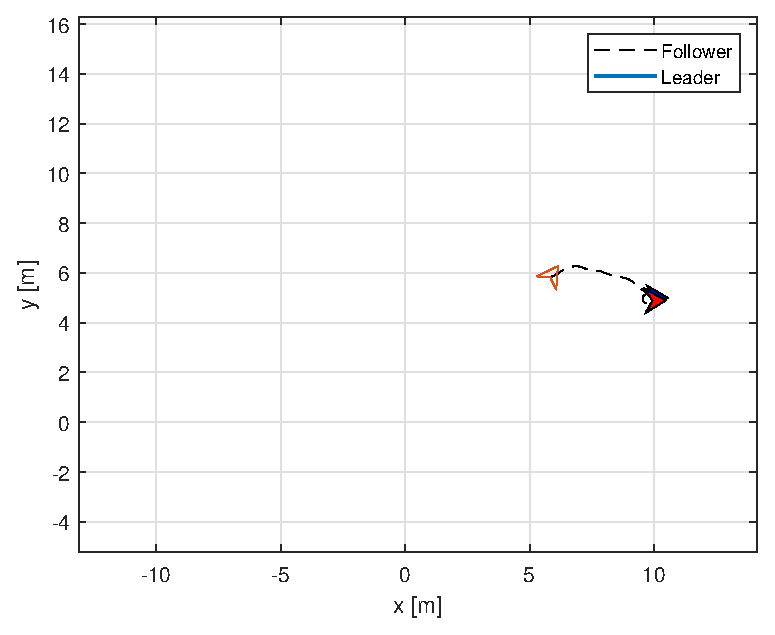
\includegraphics[scale=0.4]{figs/matlab/actorCritic/caseStudy1/trajectory.eps}
\caption{Trajectory}
\end{figure}
\end{column}

\begin{column}{0.5\textwidth}
\begin{center}

\begin{figure}
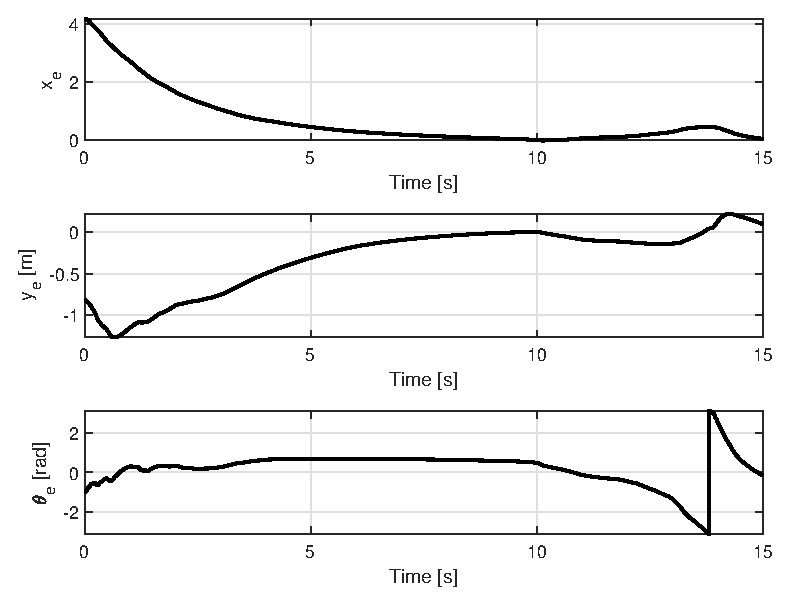
\includegraphics[scale=0.4]{figs/matlab/actorCritic/caseStudy1/error.eps}
\caption{follower position error}
\end{figure}
\end{center}

\end{column}

\end{columns}

\end{frame}
%------------------------------------------------------------------
\begin{frame}{Results}{Case Study 1}
\begin{columns}
\begin{column}{0.5\textwidth}
\begin{figure}
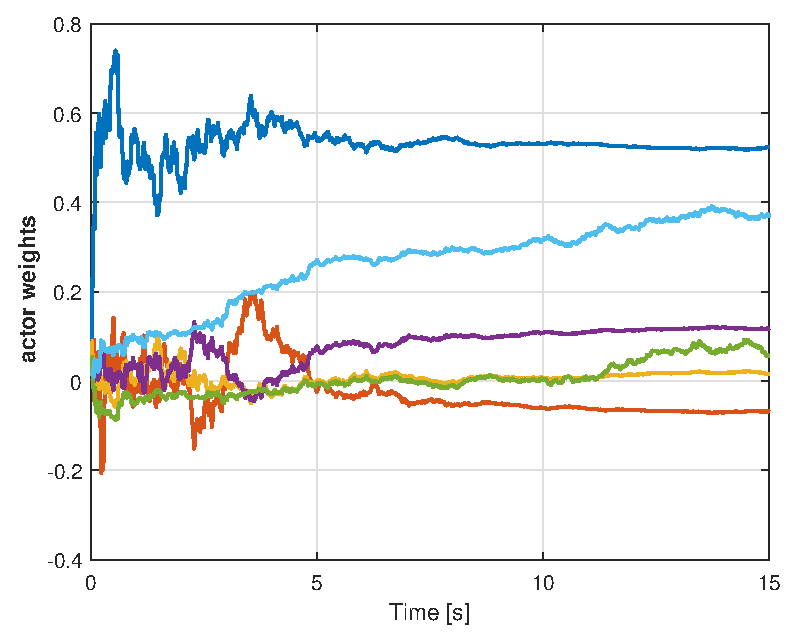
\includegraphics[scale=0.4]{figs/matlab/actorCritic/caseStudy1/weightActor.eps}
\caption{Actor Weights}
\end{figure}
\end{column}

\begin{column}{0.5\textwidth}
\begin{center}

\begin{figure}
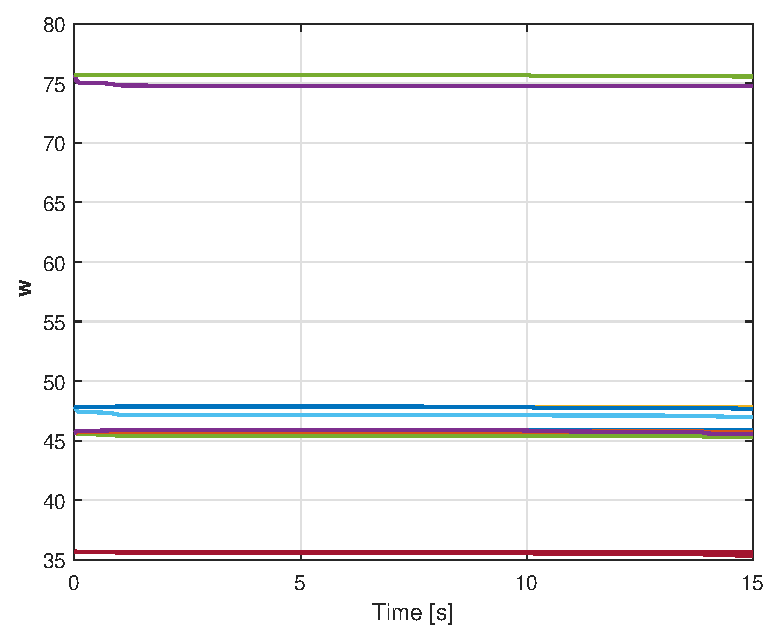
\includegraphics[scale=0.4]{figs/matlab/actorCritic/caseStudy1/weightCritic.eps}
\caption{Critic Weights}
\end{figure}
\end{center}

\end{column}

\end{columns}

\end{frame}

%------------------------------------------------------------------
\begin{frame}{Results}{Case Study 2}
\begin{columns}
\begin{column}{0.5\textwidth}
\begin{figure}
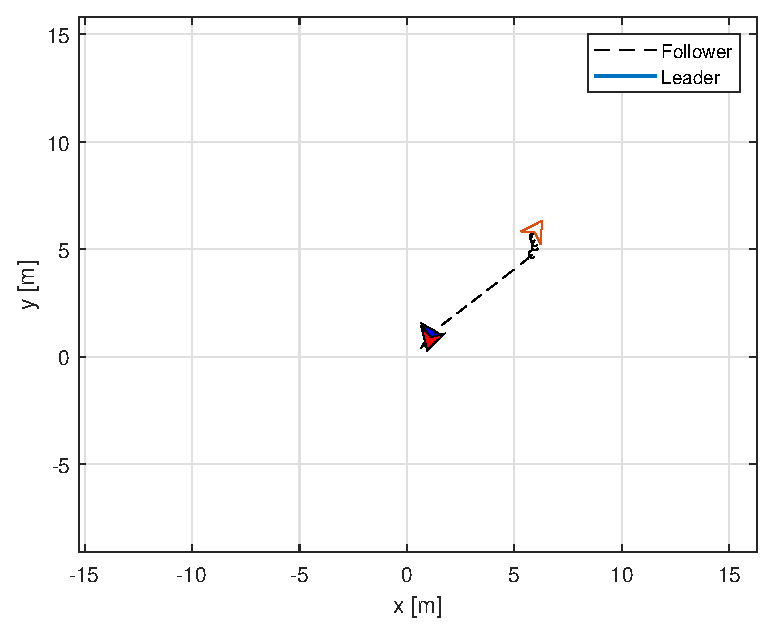
\includegraphics[scale=0.4]{figs/matlab/actorCritic/CaseStudy2/trajectory.eps}
\caption{Trajectory}
\end{figure}
\end{column}

\begin{column}{0.5\textwidth}
\begin{center}

\begin{figure}
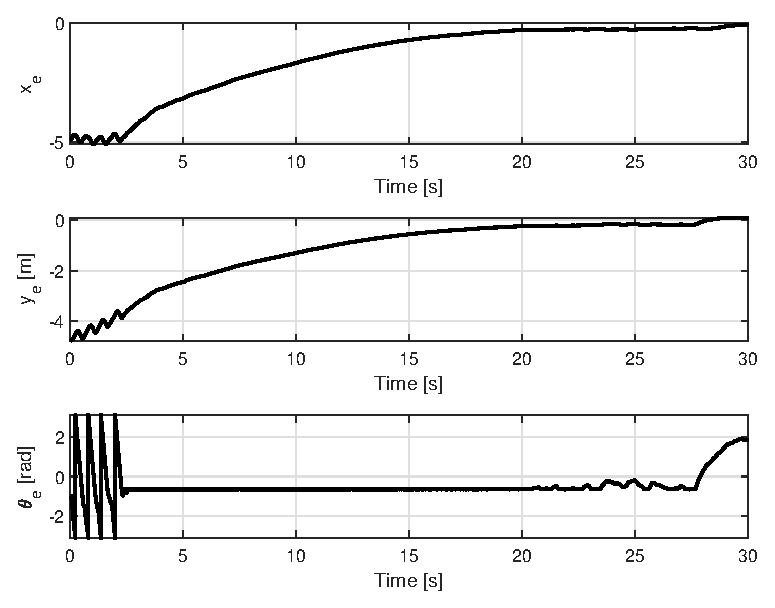
\includegraphics[scale=0.4]{figs/matlab/actorCritic/CaseStudy2/error.eps}
\caption{follower position error}
\end{figure}
\end{center}

\end{column}

\end{columns}

\end{frame}
%----------------------------------------------------------
\begin{frame}{Results}{Case Study 2}
\begin{columns}
\begin{column}{0.5\textwidth}
\begin{figure}
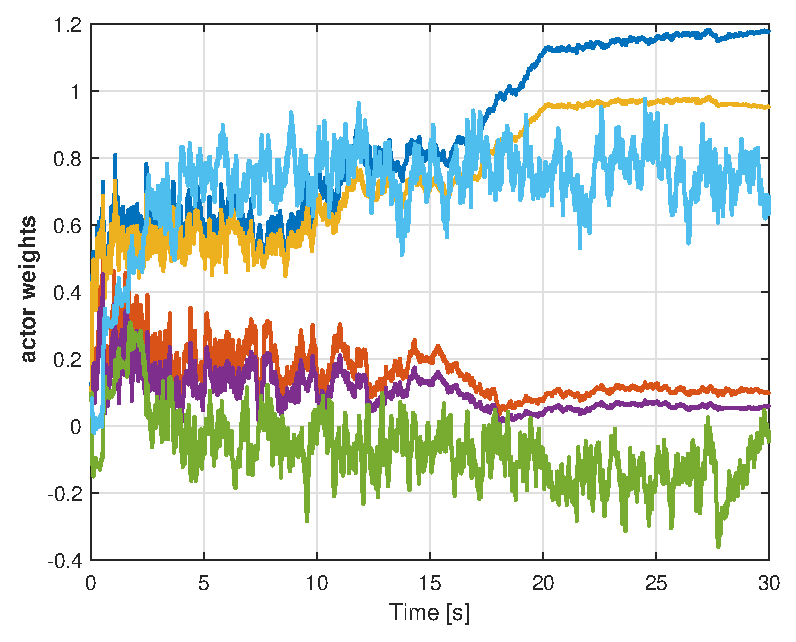
\includegraphics[scale=0.4]{figs/matlab/actorCritic/CaseStudy2/weightActor.eps}
\caption{Actor Weights}
\end{figure}
\end{column}

\begin{column}{0.5\textwidth}
\begin{center}

\begin{figure}
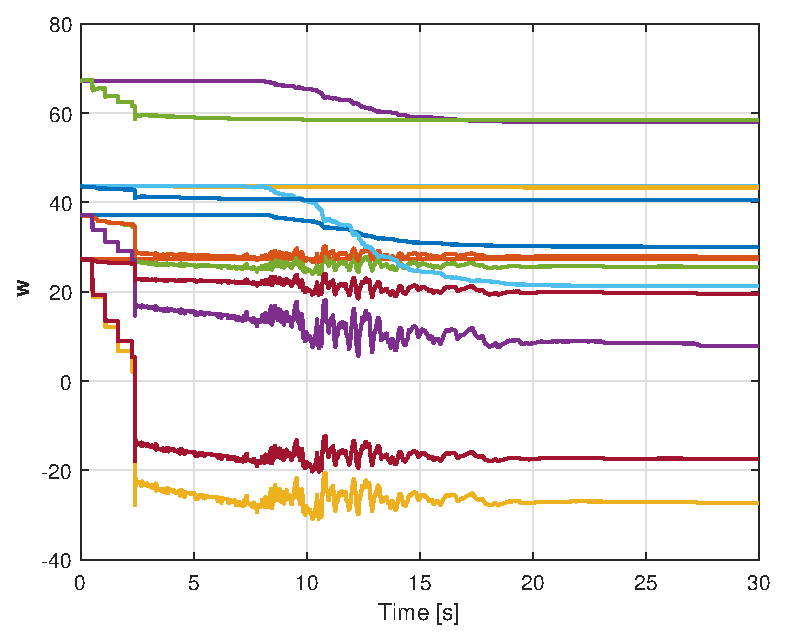
\includegraphics[scale=0.4]{figs/matlab/actorCritic/CaseStudy2/weightCritic.eps}
\caption{Critic Weights}
\end{figure}
\end{center}

\end{column}

\end{columns}

\end{frame}
%-----------------------------------------------------------------
\begin{frame}{Comments and Observations}{Gradient Descent}
\begin{block}{}
it was found that the solution still depends on a certain weights matrix , the actor critic neural network achieved promising results in different scenarios even with adding random noise to the inital p matrix
\\

\end{block}
\end{frame}
%------------

%------------
%----------------------------------
\section*{Questions}
\begin{frame}
\begin{LARGE}
\begin{center}
Questions?
\end{center}
\end{LARGE}
\end{frame}
%-----------------------
\end{document}








	